\chapter{Introduction}
\index{Introduction@\emph{Introduction}}%

\section{Introduction and Motivation}
Hurricanes are a growing concern in the operation of power grids in coastal areas. This is due partly to the increasing density of cities in coastal areas, but also due to climate change causing rising sea levels that may exacerbate impacts of flooding from hurricanes. Combined with the effects of climate change directly, there is also the indirect effect of water warming causing more frequent and more severe hurricanes \cite{MannEA2006}. This phenomenon suggests that careful power grid resilience and planning for hurricanes will be of increased importance in the coming years.

This thesis explores the gap in existing literature where previous efforts have not explicitly considered how multiple networks depended on each other for the logistics of repair, particularly the post-disaster infrastructure recovery interactions between power grid and road networks. For example, to repair a damaged power grid element, the element must be accessible to the crew attempting to repair it. Moreover, the crew will take time to go from one element to the next to repair, affecting the rate of restoration of the power grid's performance during recovery as time is lost in transit. This implies that the road network becomes part of the overall recovery efforts. This includes multiple aspects such as logistics, relief supply delivery, and power grid repair. During a hurricane, the road network will sustain substantial damage from flooding and/or debris on the road surface, which necessitates road grid repairs/clearance as well. To handle the issues of repairing power grids in a way that minimizes the amount of disruption to power service, both types of repairs (road network and power grid) should be considered jointly. To capture the interaction effects of these two networks, we consider the route that repair crews take on the road network as they conduct repairs to either the roads or the power grid. Previous literature does not study this specific interaction as discussed in the section below.

Understanding of repair efforts on power grids begins with understanding the basics of power grid topology. We divide the power grid into transmission and distribution networks. Transmission networks consist of generators, buses/substations, and high voltage connecting lines. Because this side of the grid has multiple sources and sinks, power is not guaranteed to flow in a certain direction. The distribution side of a network begins at the bus/substation level and connects end users of power to the grid as a whole. Because power flows from the substation to the end user in a single source network, these networks are comparatively simpler to model. For the sake of this thesis, we restrict ourselves to the transmission level power grids as distribution grids are simpler at an electrical level as well as being geographically small enough that ignoring the time costs that come from routing the travel of crews leads to a solution that does not stray from optimality very far. In addition, as distribution level damage happens in routine storms, power utilities have a better understanding of how to handle this damage due to experience. The scale of service loss following damage to the power grid is dramatically different in distribution and transmission. Loss of distribution power lines can lead to loss of power service to small segments of a neighborhood while loss of a substation or set of transmission lines can knock out power to several neighborhoods or entire towns depending on the extent of redundancies.


\section{Literature Review}
\subsection{Hurricane Damage Modeling}
When delving into the background literature, no discussion of modeling repair after a hurricane can happen before looking at the literature on damage to power grids from hurricanes. Guikema et al. \cite{GuikemaEA2010} use a model based on negative binomial regression to estimate the number of downed power lines. They combine this with a classification tree that handles flooding and wind speed as a secondary method for estimation of damage severity. Scherb et al. \cite{ScherbEA2015} on the other hand take an approach more rooted in scenario generation and they try to use the peak wind speed and proximity to the eye wall of a hurricane to construct a loss function (a function that maps wind speed onto probability of damage for a given element) for power lines. Figure 1.1  provides an example of the loss function that shows the relationship between probability of varying levels of damage and local peak windspeed during the hurricane. In their figure $\mu$ and $\sigma$ are respectively the mean and standard deviation of number of breakages in a line for each level of damage.

Both of these papers come to the similar conclusion that damage to 40-70\% of the power lines in the network due to wind and thrown debris is common in hurricanes. Damage is geographically distributed based on proximity to the eye-wall of a hurricane, but because hurricanes are frequently hundreds of miles across, damage inside of a single city may appear functionally random due the small geographic area highly similar peak wind speeds. 

\begin{figure}[htbp]
	\centering
	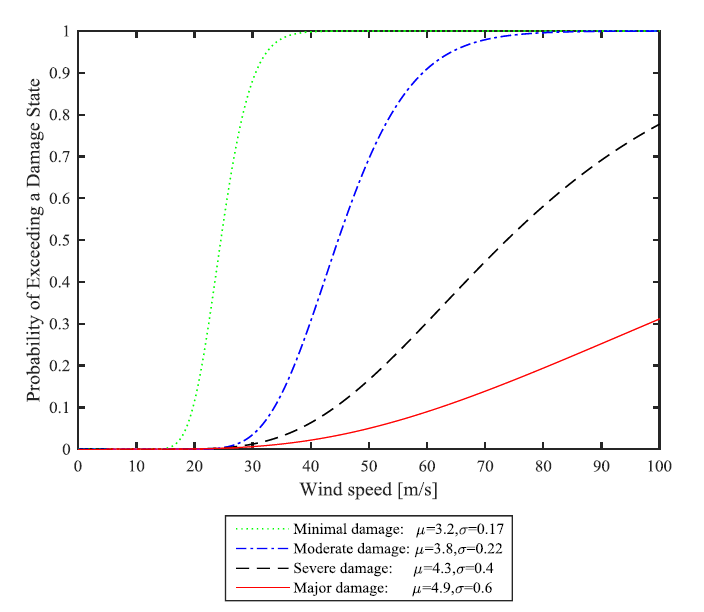
\includegraphics[width=.5\linewidth]{ScherbFigure.PNG}
	\caption{A power line loss function example from \cite{ScherbEA2015}}
\end{figure}

Winkler et al. \cite{WinklerEA2010} provide the most thorough analysis of these 3 papers using real world topographies from various small regions of Texas and generating loss functions for both lines and substations. Worth noting in all three of these examples is that lines and substations sustain the most damage, but generators themselves are robust enough that a hurricane is unlikely to damage them directly, though they may sustain disruption to operations because of disrupted fuel or crew availability. This means they can be treated as undamaged in terms of generation capacity in the modeling in later sections as the generator's functionality depends on its associated substation connecting it to the grid. 
\subsection{Existing Power Grid Repair Modeling}
Repair of power grids in the wake of hurricanes is a reasonably well studied area of research. Ang \cite{NPSMasters} solves a scheduling problem of power grid repair in the wake of both hurricanes and terrorist attacks. The problem is determining in which order should elements be repaired with little consideration of the actual logistics of getting crews to the sites where power grid repair can happen. While they do not consider impacts of roads, they focus on extending repair models to DC power flow based models of the power grid when covering how to model a damaged power grid. Along similar lines, Arab et al. \cite{ArabEA2015} solve a similar problem under uncertainty by treating the state of each power line and generator as a random Bernoulli variable and solving the ensuing stochastic optimization problem. Though it solves the problem as a two stage stochastic program with recourse and treatment of the hurricane damage much closer resembles empirical damage, there is still no consideration of repair logistics, only scheduling and inventory amount. 

Ouyang and Duenas-Osorio \cite{OuyangEA2014} do a statistical analysis of the rate at which damage is recovered in the context of broader power grid resilience. While more descriptive than prescriptive, their analysis concludes that transmission grid repairs take priority alongside ``critical facilities vital to public safety, health, and welfare". Of note in this paper is that their observation that much of the existing literature on repairs to power grid is based on descriptive studies of statistical repair times rather than model-driven optimization models for how to improve that process.

Golari et al. \cite{GolariEA2014} take a different approach to ensuring power demand satisfaction in the context of a damaged power network by approaching the problem in the lens of construction of sub-grids (termed ''islands" in much of the electrical engineering literature) in order to keep demand satisfied. This is done by solving a two stage stochastic program in order to identify the best sub-grids to construct under the uncertainty of a set of contingencies. Islanding is an active field of study in power grid engineering for developing tools to minimize the impact of disaster damage. Panteli et al. \cite{Panteli2016} study disaster damage by constructing islanding plans in a way that would minimize load loss subject to severe weather. Though there is no consideration of repair, their modeling warrants the importance of resilience as an area of study.  A follow on paper to that by Nobels and Panteli \cite{NobelsEA2019} extends the previous work on resilience from islanding  by using IEEE 30 and 57 bus test networks to analysis of cascaded failures caused by disasters. In addition, their modeling differentiates intentional vs unintentional load shedding due to the disaster and corresponding response.
\subsection{Existing Road Grid Repair Modeling}
Pregnolato et al. \cite{PregnolatoEA2017} provide an overview of probability of road damage by location and intensity of damage to the road in terms of flooding and debris. They go on to provide a literature review and meta-analysis of existing papers in this subfield. In addition, the paper summarizes a variety of versions of flooding depth-disruption functions for roads based on local rain intensity. The focus of this paper is not modeling repair efforts as the models provided for road repair are cursory, but the analysis of damage to road networks from debris and flooding in the wake of a disaster is covered in depth.

Looking next at how previous papers have addressed modeling flooding and how to interact with it in a repair context, we start with a paper by Duque et al. \cite{DuqueEA2016}. This paper focuses on distribution of relief supplies, but in the context of the problem of supply distribution the paper considers repair of flooded or damaged roads. Though they solve the problem with dynamic programming rather than the mixed integer programming of similar papers; the idea of repair of roads by traversing them at additional cost is the main contribution of their modeling approach.

Also of note from the perspective of road repair is a paper by Aksu and Ozdamar \cite{AksuEA2014}. Again, it is not a paper focused focused on direct repair of networks, but rather focuses on evacuation and accessibility to areas flooded by the a disaster. This provides additional insight into flooding and relief as well as a different treatment of the problem using mixed integer programming rather than the dynamic programming of Duque et al. Both of these treatments cover short term road clearance in the context of disaster response and relief. 

All three of these papers make similar assumptions in that minor damage to road networks can be repaired in a time horizon relevant to immediate post-disaster response. While more severe damage to roads can require resurfacing or replacement of bridges, debris and flooding clearance is distinct from those repairs.

\subsection{Resilience}
As this thesis deals partly with resilience, we look to the corresponding literature for definitions of resilience in the context of disaster response for power grids. Molyneaux et al. \cite{MolyneauxEA2016} provide a multi-disciplinary literature review of power grid resilience. They broadly define resilience as ``capacity to cope with the unexpected". While they go through multiple measures for resilience they use primarily metrics of price. For example, they reduce power flow to the cost of power and the change in cost from the hurricane damaging the network rather than treating the utility of unsatisfied power demand directly. This approach can be very useful, but it ignores that power is more valuable to some consumers than others in the wake of a hurricane. For example, a hospital restoring power is likely more valuable than a factory restoring power. Panteli and Mancarella \cite{Panteli2017} focus on more specific resilience definitions in the context of disaster response. They focus on both magnitude of drop in service of power demand as well as time dependent total loss of power demand satisfied.

Much of the literature on resilience for power grids comes from study of protecting the power grid from directed attacks. Fortification against a potential terrorist attack is a standard form of study for grid resilience and appears in much of the literature. Relevant among these is a paper by Deka et al. \cite{Deka2018} which provides a study of both initial damage as well as potential damage stemming from cascading failures. In addition, they identify  elements crucial to construction of resilient power networks. More relevant to this thesis is work by Salmeron et al. \cite{Salmeron2004} Their work identifies key elements to make resilient using mixed integer programming based on a DC-powerflow based model of power grids. They solve a bilayer optimization model that involves minimization of the maximum power demand that can be satisfied to determine optimal interdiction. The inner problem how to maximize the amount of power demand that can be serviced given the state of the power grid under damaged operations. The outer problem is therefore how to choose power grid damage in order to make sure that as little demand can be satisfied under ideal operation of the damaged network. This interaction between attacker and defender provides the framework from which they plan resilience.

